% Per-node sidecar load vs. agents per node (E3c, live 8-node sweep).
% Two separate axes rather than one with two y-scales: CPU (%) and RSS (MB)
% are different units, and a dual-axis plot would invite a false comparison.
% Both axes start at zero, so "flat" reads as flat rather than as an
% artefact of a truncated baseline.
%
% Data: scripts/eval/out/e1d_sidecars_k{1,2,4}.csv (collector process),
% cross-checked against the E3c table in scripts/eval/out/results.md.
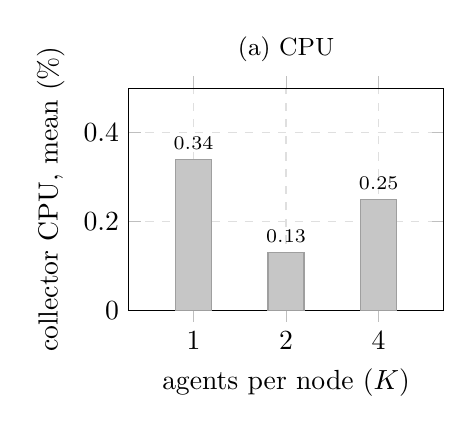
\begin{tikzpicture}
\begin{axis}[
    width=0.46\linewidth, height=4.4cm,
    ybar, bar width=13pt,
    xlabel={agents per node ($K$)}, ylabel={collector CPU, mean (\%)},
    symbolic x coords={1,2,4}, xtick=data,
    ymin=0, ymax=0.5,
    nodes near coords, every node near coord/.append style={font=\scriptsize, text=black},
    grid=major, grid style={dashed,gray!25},
    tick style={draw=gray!50},
    enlarge x limits=0.35,
    title style={font=\small}, title={(a) CPU},
]
\addplot[fill=gray!45, draw=gray!75, mark=none] coordinates {(1,0.34) (2,0.13) (4,0.25)};
\end{axis}
\end{tikzpicture}
\hfill
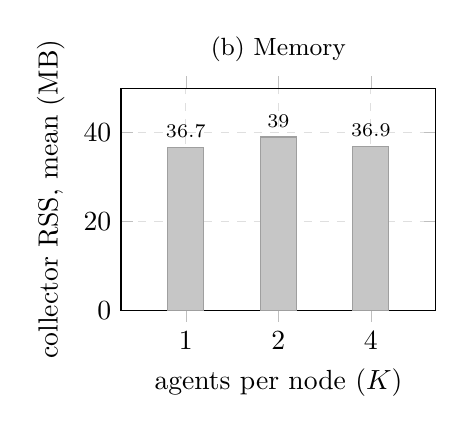
\begin{tikzpicture}
\begin{axis}[
    width=0.46\linewidth, height=4.4cm,
    ybar, bar width=13pt,
    xlabel={agents per node ($K$)}, ylabel={collector RSS, mean (MB)},
    symbolic x coords={1,2,4}, xtick=data,
    ymin=0, ymax=50,
    nodes near coords, every node near coord/.append style={font=\scriptsize, text=black},
    grid=major, grid style={dashed,gray!25},
    tick style={draw=gray!50},
    enlarge x limits=0.35,
    title style={font=\small}, title={(b) Memory},
]
\addplot[fill=gray!45, draw=gray!75, mark=none] coordinates {(1,36.7) (2,39.0) (4,36.9)};
\end{axis}
\end{tikzpicture}
